\documentclass[12pt,runningheads]{article}
\usepackage[utf8]{inputenc}

%enable apa
\usepackage[british]{babel}
\usepackage{csquotes}
\usepackage[backend=biber,style=apa]{biblatex}
\DeclareLanguageMapping{british}{british-apa}

%some additional packages
\usepackage[pdftex]{graphicx}

\addbibresource{references.bib}

\begin{document}

\title{Algorithms and Data Structure Project\\Elementary Graph Algorithms}
\author{Himani Tokas}
\maketitle

%text goes here
\section{Introduction}
Graphs can be directed or un-directed networks. A graph is represented as G(V,E), where 'E' represent edges and 'V' represent vertices of the graph.Depth First Search and Breadth First Search are two elementary graph algorithms.


\subsection{Idea of Depth First Search}
Its idea is to search deeper in the tree/adjacency list.Depth-first search explores edges out
of the most recently discovered vertex v that still has unexplored edges leaving it.
Once all of v’s edges have been explored, the search “backtracks” to explore edges
leaving the vertex from which v was discovered. This process continues until we
have discovered all the vertices that are reachable from the original source vertex.
If any undiscovered vertices remain, then depth-first search selects one of them as
a new source, and it repeats the search from that source. The algorithm repeats this
entire process until it has discovered every vertex.
\subsection{Idea of Breadth First Search}
Given a graph G(V,E) and a distinguished source vertex s, breadth-first
search systematically explores the edges of G to “discover” every vertex that is
reachable from s. It computes the distance (smallest number of edges) from s
to each reachable vertex. It also produces a “breadth-first tree” with root s that
contains all reachable vertices. For any vertex v reachable from s, the simple path
in the breadth-first tree from s to v corresponds to a “shortest path” from s to v
in G, that is, a path containing the smallest number of edges. The algorithm works
on both directed and undirected graphs.
\subsection{Graph Representation}
\subsubsection{Undirected Graph Representation}
An undirected graph does not have any arrows. It looks as follow:

\begin{figure}[htp]
    \centering
    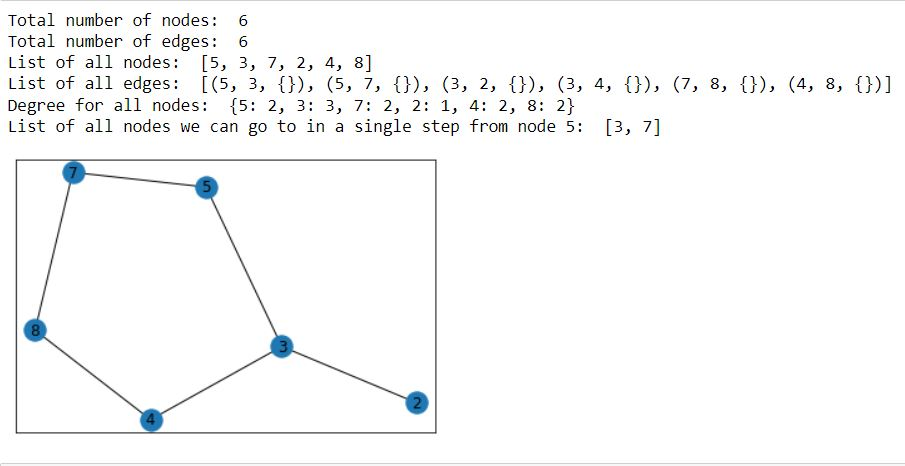
\includegraphics[width=12cm,height=12cm]{undirectedgraph.JPG}
    \caption{An undirected graph with 6 vertices and 6 edges}
    \label{fig:galaxy}
\end{figure}
\subsubsection{Directed Graph Representation}
An directed graph have arrows. It looks as follow:

\begin{figure}[htp]
    \centering
    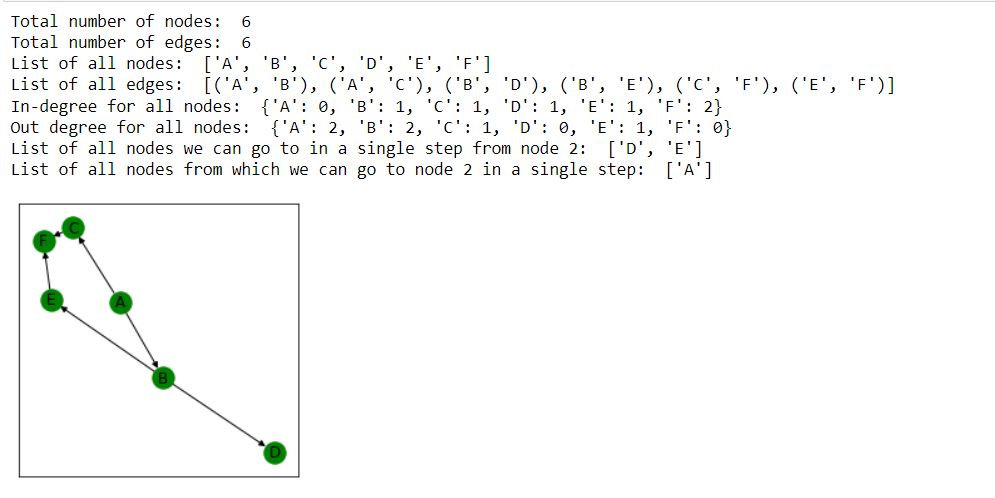
\includegraphics[width=12cm,height=12cm]{directedgraph.JPG}
    \caption{A directed graph with 6 vertices and 6 edges}
    \label{fig:galaxy}
\end{figure}
\section{Methodology}
For analyzing the algorithm more than one graph is required. Since, it is not possible to create adjacency lists randomly, first adjacency matrices of size varying from $10\times 10$ to $2000\times 2000$ were generated and converted into adjacency lists. The function where adjacency list is being created call the depth first search and breadth first search functions to solve these algorithms and returns back the output.
\section{Data used to study Depth First Search Time Complexity}
\subsection{Data}
Random adjacency matrices of size varying from $10\times 10$ to $2000\times 2000$ were generated and converted into adjacency lists. A total of 199 data points are used to find time complexity:

\begin{figure}[htp]
    \centering
    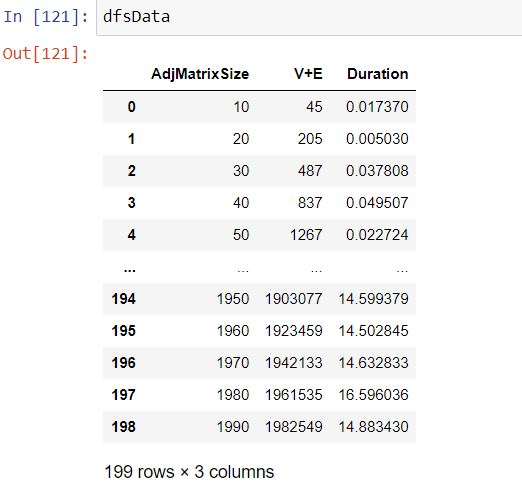
\includegraphics[width=12cm,height=10cm]{dfsdata.JPG}
    \caption{Data points for depth first search analysis: V+E represent sum of vertices and edges and Duration is the time taken to evaluate the particular adjacency list.}
    \label{fig:galaxy}
\end{figure}

\section{Time Complexity of Depth First Search Algorithm}
Time complexity is given as O(V+E) because we are visiting every edge, traversing through all vertices. 
\subsubsection{Time Complexity found through data regression}
\begin{figure}[htp]
    \centering
    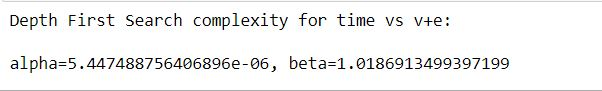
\includegraphics[width=12cm]{dfscomplexity.JPG}
    \caption{Beta value for time complexity is approximately 1.01. If we get more data points it will be more closer to 1.Hence time complexity for DFS is O(V+E).}
    \label{fig:galaxy}
\end{figure}
\subsubsection{Regression Graph}
Following curve is obtained for duration versus sum of vertices and edges for DFS.Data points were increased to 790 to get a better visual.

\begin{figure}[htp]
    \centering
    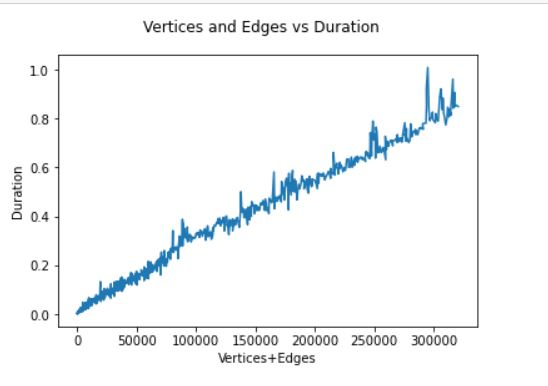
\includegraphics[width=8cm]{dfsgraphline1.JPG}
    \caption{DFS plot for duration and number of edges and vertices. Total data points on graph is 790}
    \label{fig:galaxy}
\end{figure}
\section{Application of Depth First Search from CLRS Book}
\subsection{Topological Sort}
A topological sort of dag(directed a-cyclic graph) G(V,E) is linear ordering of all its vertices such that if G contains an edge (u,v) then u must come before v.
Following problem is given in the book:
\begin{figure}[htp]
    \centering
    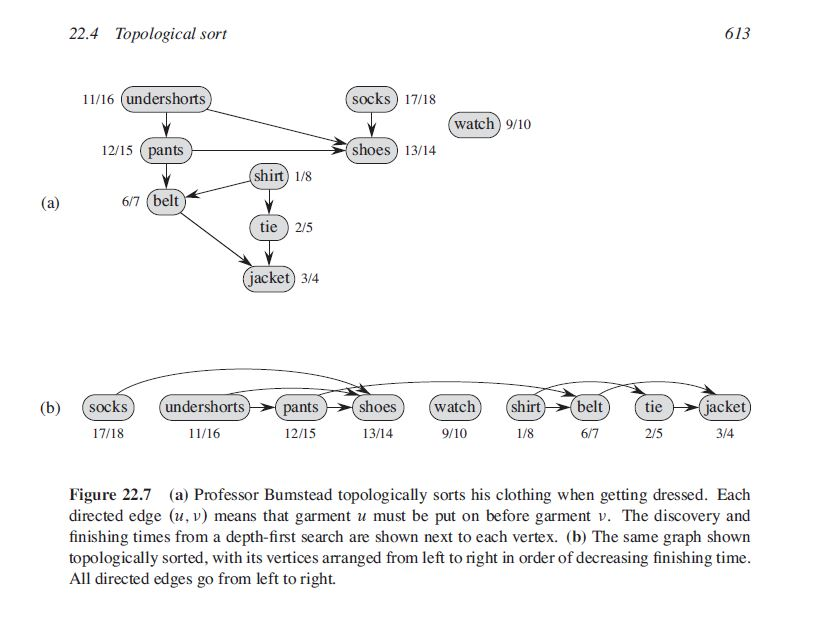
\includegraphics[width=10cm]{topologicalsortproblem.JPG}
    \caption{From fig(a) an adjacency list is created and DFS is applied to find (b) as output.}
    \label{fig:galaxy}
\end{figure}
\subsubsection{Adjacency List }
Following Adjacency List is formed from fig(a):
\begin{figure}[htp]
    \centering
    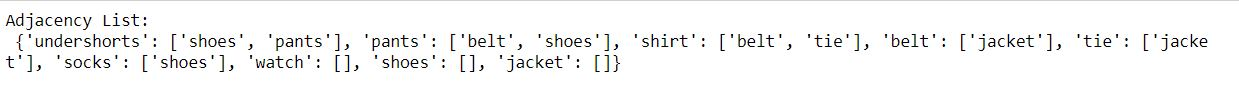
\includegraphics[width=10cm]{topadjlist1.JPG}
    \caption{Adjacency List in form of a python dictionary}
    \label{fig:galaxy}
\end{figure}
\subsubsection{Execution: Starting from 'Undershorts'}
Following sorted order is obtained if we start sorting from 'undershorts' using DFS:
\begin{figure}[htp]
    \centering
    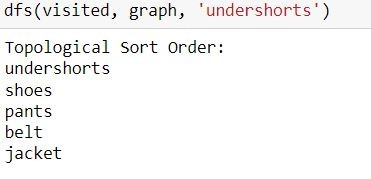
\includegraphics[width=6cm]{topsort.JPG}
    \caption{Topological Sort starting from 'undershorts'. Different sorted orders will be obtained if we change the starting point.}
    \label{fig:galaxy}
\end{figure}
\section{Data Used for Breadth First Search Analysis}
Adjacency matrices order varying from $10\times 10$ to $300\times 300$ were converted into adjacency lists. A total of 290 data points are used:
\begin{figure}[htp]
    \centering
    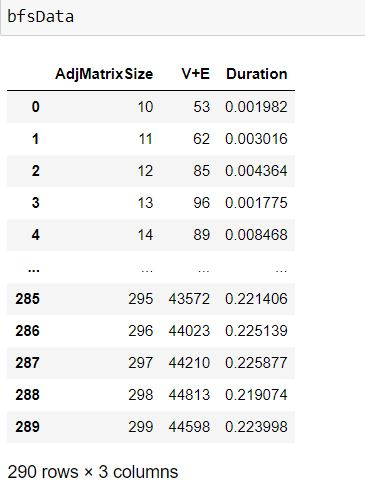
\includegraphics[width=4cm]{bfsdata.JPG}
    \caption{Data for breadth first search analysis}
    \label{fig:galaxy}
\end{figure}
\\
\\
\section{Time Complexity for BFS Algorithm}
It is also given as O(V+E), similar to DFS.
\subsubsection{Time Complexity found through data regression}
\begin{figure}[htp]
    \centering
    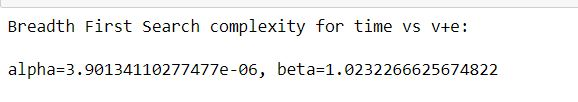
\includegraphics[width=12cm,height=3cm]{bfsregression.JPG}
    \caption{Beta value is closer to 1, hence time complexity is O(V+E)}
    \label{fig:galaxy}
\end{figure}
\subsubsection{Data Regression Graph}
\begin{figure}[htp]
    \centering
    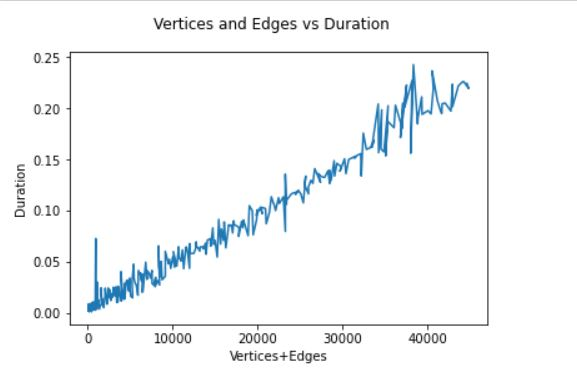
\includegraphics[width=12cm]{bfslinegraph.JPG}
    \caption{This graph is obtained if we plot duration and sum or vertices and edges.}
    \label{fig:galaxy}
\end{figure}
\section{References}
\begin{enumerate}
    \item Book: CLRS (Thomas H. Cormen, Charles E. Leiserson, Ronal L. Rivest, Clifford Stein): Introduction to Algorithms, Third Edition
    \item https://stackoverflow.com/
\end{enumerate}
\printbibliography

\end{document}
